%T
% https://github.com/matze/mtheme
\documentclass[10pt]{beamer}

\usetheme[progressbar=frametitle]{metropolis}

\usepackage{booktabs}
\usepackage[scale=2]{ccicons}
\usepackage{graphicx}
\graphicspath{ {images/} }	%resim dosyalari klasörü

\usepackage{pgfplots}
\usepgfplotslibrary{dateplot}

\usepackage{xspace}
\newcommand{\themename}{\textbf{\textsc{metropolis}}\xspace}

\title{Yuksek Guc Yogunluklu Donusturuculer}
\subtitle{Zero-Voltage-Switching PWM Resonant Full-Bridge
	Converter With Minimized Circulating Losses and
	Minimal Voltage Stresses of Bridge Rectifiers for
	Electric Vehicle Battery Chargers
	}
\date{\today}
\author{NAZIM YILDIZ}
\institute{Elektrik-Elektronik}
\titlegraphic{\hfill
\includegraphics[height=1.5cm]{pau_logo.jpg}}

\begin{document}

\maketitle

\begin{frame}{Table of contents}
  \setbeamertemplate{section in toc}[sections numbered]
  \tableofcontents[hideallsubsections]
\end{frame}

\section{Topoloji Tanitimi}

\begin{frame}[fragile]{Topoloji Incelemesi}

   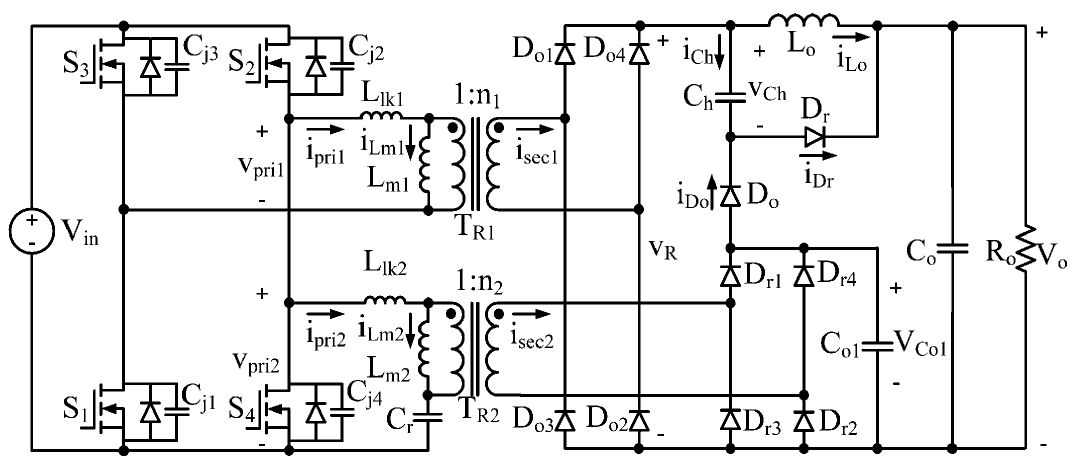
\includegraphics[scale=0.3]{sema.png}

  $T_{R1}$ FullBridge\newline
  $T_{R2}$ LLC

\end{frame}


\section{Analiz}
\begin{frame}{Mode Incelemesi}
	\begin{figure}
		\centering
		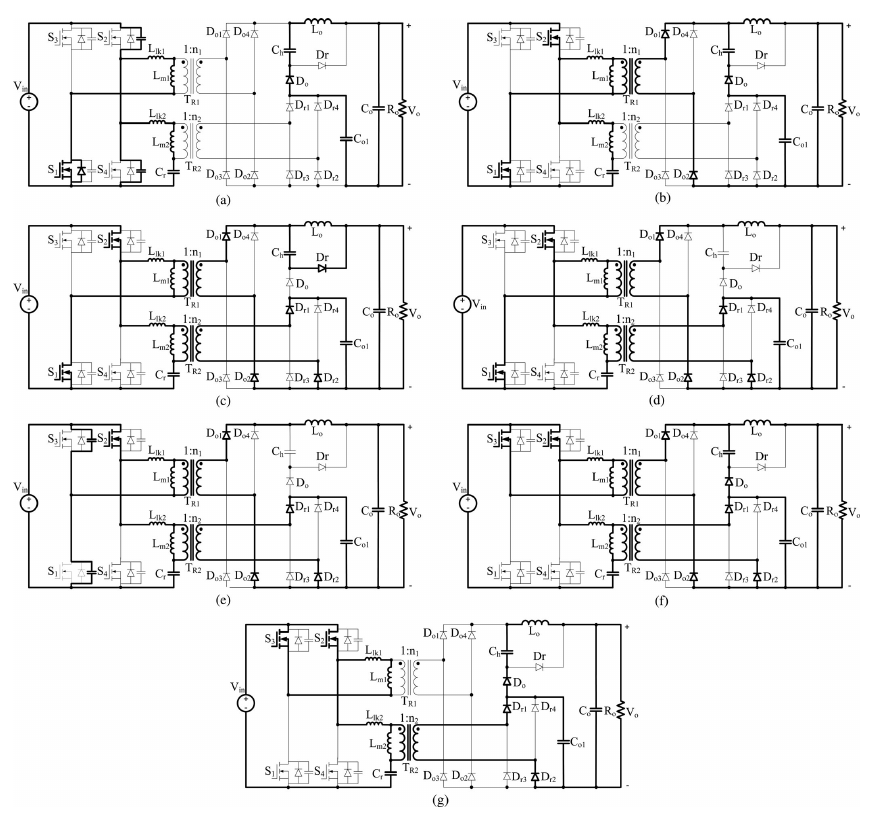
\includegraphics[scale=0.25]{modes.png}
	\end{figure}

\end{frame}

\begin{frame}{Mode1}
	\begin{figure}
		\centering
		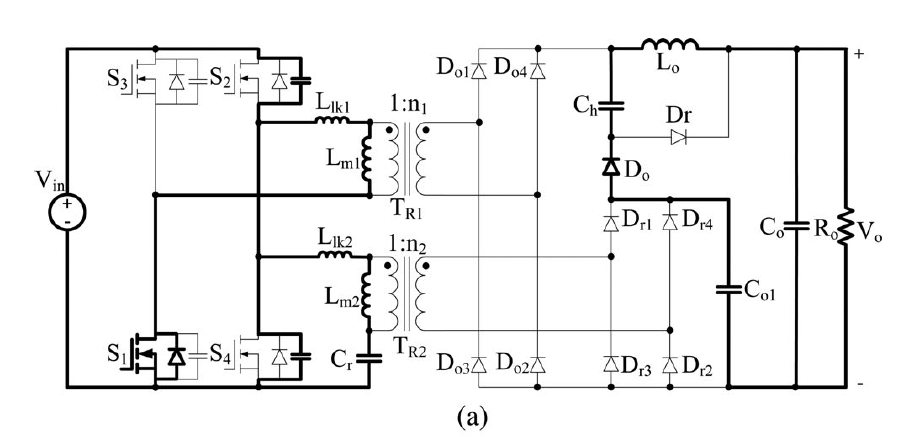
\includegraphics[scale=0.30]{mode_a.png}
	\end{figure}
	\begin{itemize}
		\item $T_{R1}$ ve $T_{R2}$ miknatislama akimlari primer tarafinda dolasirlar.
		\item $i_{LM2}$ akimi $C_{S4}$ ve $C_{S2}$ sirasiyla sarj ve desarj eder.
		\item Olu zamanin ardindan $S_{2}$ ZVS ile iletime gecer.
	\end{itemize}
\end{frame}

\begin{frame}{Mode2}
	\begin{figure}
		\centering
		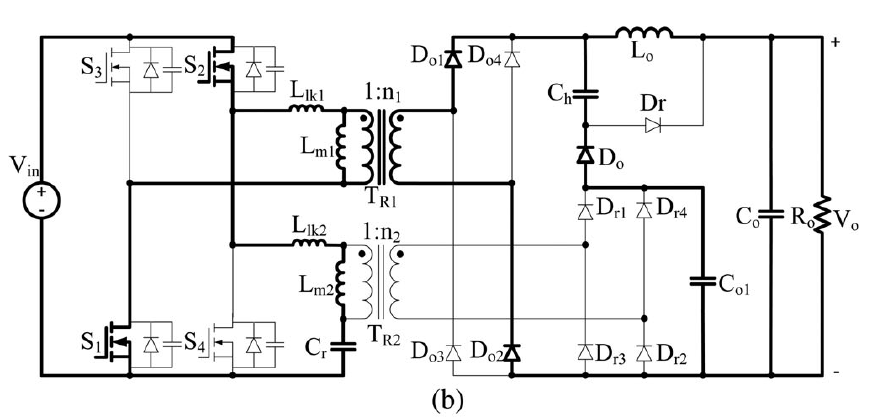
\includegraphics[scale=0.30]{mode_b.png}
	\end{figure}
	\begin{itemize}
		\item $i_{pri1}$ akimi $i_{Lm1}$ miknatislama akimi gecmeye baslamasiyla $T_{R1}$ cikisi beslemeye baslar. $i_{pri1}$ akimi $n_1 \times i_{Lo}$ degerine esit olana kadar dogrusal artar.
 		\item $i_{sec1}$ halen $i_{Lo}$ dan kucuktur bu nedenle $C_h$ ve $C_{o1}$ kondansatorleri cikisa enerji aktarmaya devam eder.
		\item Geleneksel PSFB primer akimi dogrusal artarken cikisa guc aktarilamadi icin kayip-duty meydana gelmektedir.
	\end{itemize}
\end{frame}

\begin{frame}{Mode3}
	\begin{figure}
		\centering
		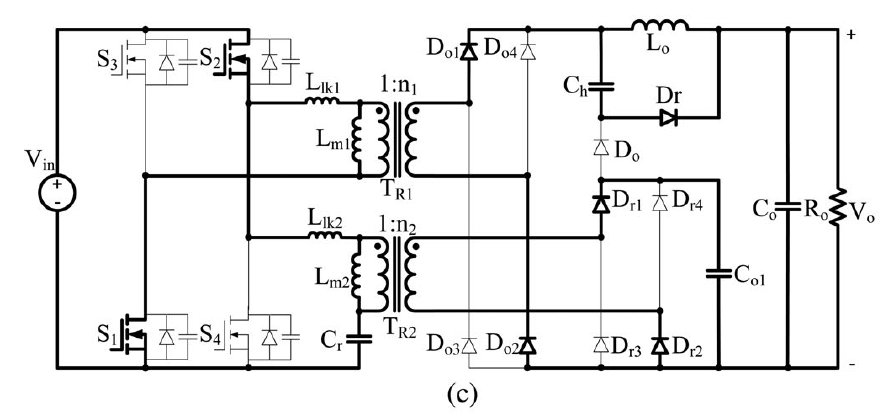
\includegraphics[scale=0.30]{mode_c.png}
	\end{figure}
	\begin{itemize}
		\item $i_{sec1}$ akimi $i_{Lo}$ daha yuksektir.
		\item $L_lk1$ ve $C_h$ arasinda rezonans baslar. Cikisa PWM ve rezonans ile olusan enerji aktarilir.
		\item LLC ise $C_{o1}$ sarj eder.
	\end{itemize}
\end{frame}

\begin{frame}{Mode4}
	\begin{figure}
		\centering
		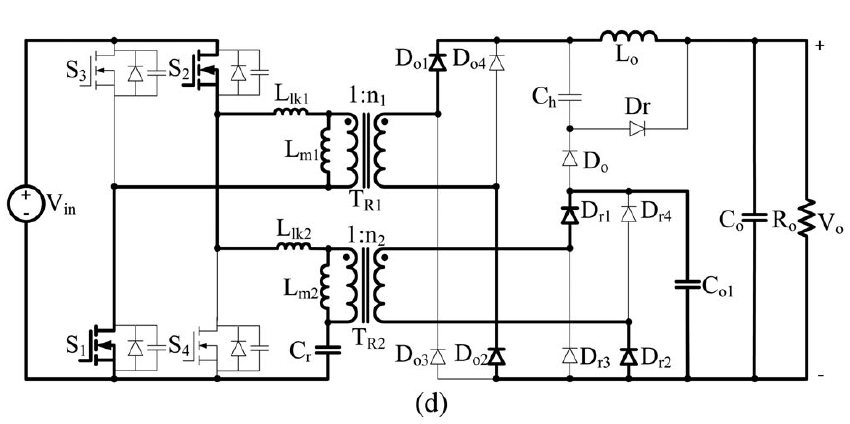
\includegraphics[scale=0.30]{mode_d.png}
	\end{figure}
	\begin{itemize}
		\item $D_r$ ZCS ile kesime girer.
		\item $i_{sec1}$ akimi $i_{Lo}$ akimina esittir ve $T_{R1}$ cikisa enerji aktarir.
		\item LLC ise $C_{o1}$ sarj eder.
	\end{itemize}
\end{frame}

\begin{frame}{Mode5}
	\begin{figure}
		\centering
		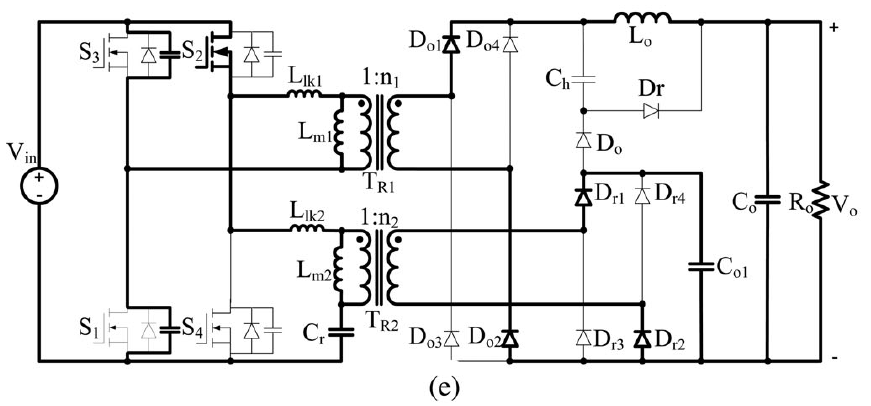
\includegraphics[scale=0.30]{mode_e.png}
	\end{figure}
	\begin{itemize}
		\item $S_1$ kesime girer. $i_{pri1}$ $C_{S1}$ ve $C_{S3}$ kondansatorlerini sirasiyla sarj ve desarj eder.
		
		\item Olu zamanin ardindan $S_3$ ZVS ile iletime girer.
	\end{itemize}
\end{frame}

\begin{frame}{Mode6}
	\begin{figure}
		\centering
		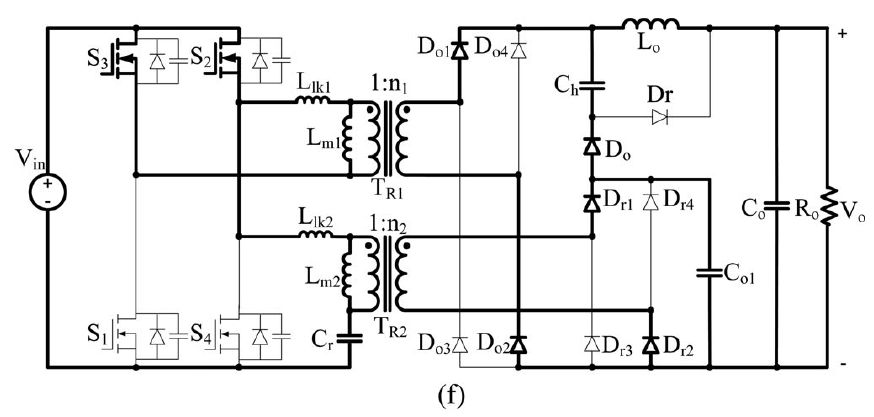
\includegraphics[scale=0.30]{mode_f.png}
	\end{figure}
	\begin{itemize}
		\item $i_{sec1}$ $<$ $i_{Lo}$ dir ve $D_o$ iletime girer.
		\item $C_h$ ve $C_{o1}$ kondansatorlerinin gerilimleri toplami $L_{lk1}$'e yansimasi sonucu $i_{pri1}$ akimi hemen resetlenir. Boylece serbest dolasim bolgesi olusmaz. Bu sırada LLC devresi $C_{o1}$ kondansatorunu sarj eder.
		\item Olu zamanin ardindan $S_3$ ZVS ile iletime girer.
	\end{itemize}
\end{frame}

\begin{frame}{Mode7}
	\begin{figure}
		\centering
		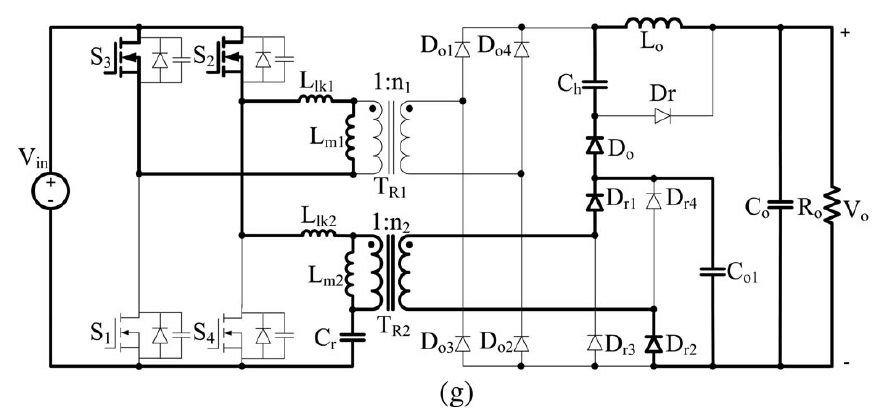
\includegraphics[scale=0.30]{mode_g.png}
	\end{figure}
	\begin{itemize}
		\item $i_{sec1}$ akimi sifirlanir ve PSFB tarafindan cikisa enerji aktarimi kesilir.
		\item $i_{Lo}$ akimi $C_h$ ve $C_{o1}$ üzerinden yolunu tamamlar. Boylece $L_o$ bobini PSFB den daha kucuk olur.
 		\item PSFB de serbest dolasim bolgesinde akim 2 diyot uzerinden dolasir. Ancak onerilen tasarimda 1 adet diyot uzerinden bobin akimi yolunu tamamlar.
	\end{itemize}
\end{frame}


\section{Deneysel Calisma ve Ciktilar}
\begin{frame}{Verim}
	\begin{figure}
		\centering
		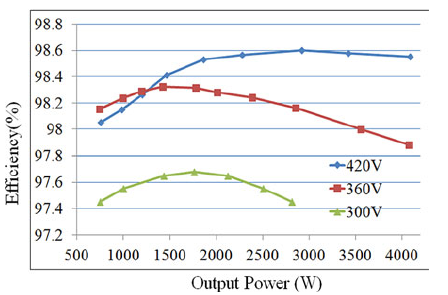
\includegraphics[scale=0.50]{efficiency.png}
	\end{figure}
	Yukaridaki grafikte 300, 360 ve 420V giris gerimleri icin verim ile cikis gucu arasindaki iliski verilmistir.
\end{frame}

\begin{frame}{Serbest Dolasim}
	\begin{figure}
		\centering
		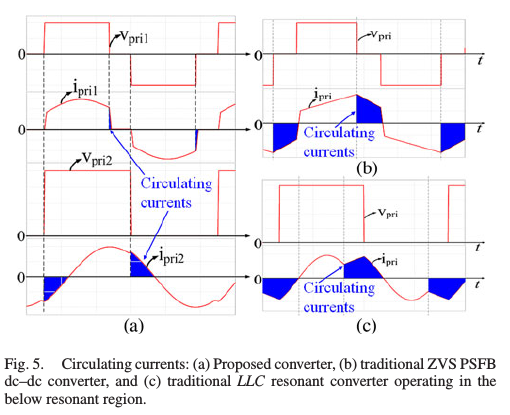
\includegraphics[scale=0.50]{circulating_currents.png}
	\end{figure}
\end{frame}

\begin{frame}{Verim}
	\begin{figure}
		\centering
		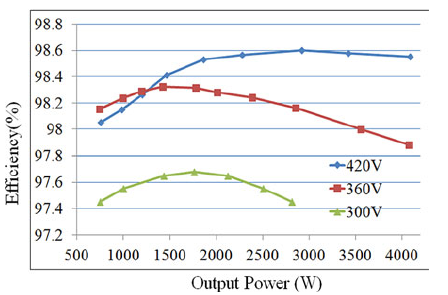
\includegraphics[scale=0.50]{efficiency.png}
	\end{figure}
	Yukaridaki grafikte 300, 360 ve 420V giris gerimleri icin verim ile cikis gucu arasindaki iliski verilmistir.
\end{frame}

\begin{frame}{Voltaj Stres}
	\begin{figure}
		\centering
		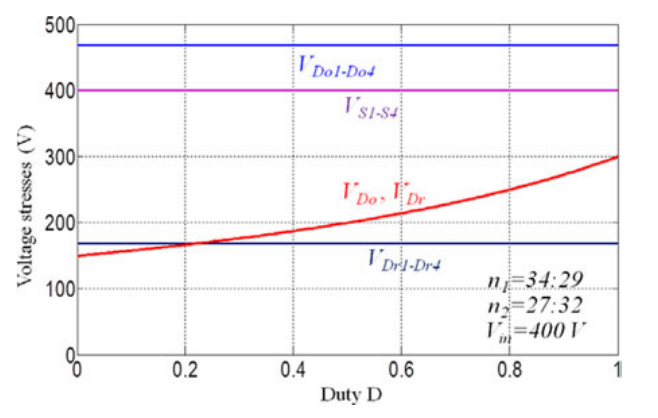
\includegraphics[scale=0.50]{voltage_stress.png}
	\end{figure}
	Yukaridaki grafikte 300, 360 ve 420V giris gerimleri icin verim ile cikis gucu arasindaki iliski verilmistir.
\end{frame}

\section{Sonuc}
\begin{frame}[fragile]{Avantajlari}
	\begin{itemize}
		\item Tum yuk araligi boyunca ZVS saglaniyor.
		\item Cikis dogrultma diyotlari voltaj sitresleri dusuk.
		\item Serbest dolasim boglesi olusmuyor.
		\item Geleneksel PSFB donusturucude meydana gelen kayip duty sorunu olusmuyor.
		\item $C_h$ ve $C_{o1}$ kondansatorleri sayesinde $L_o$ cikis bobini kuculur.
	\end{itemize}
\end{frame}	

\begin{frame}{Kritik Dalga Sekilleri}
	\begin{figure}
		\centering
		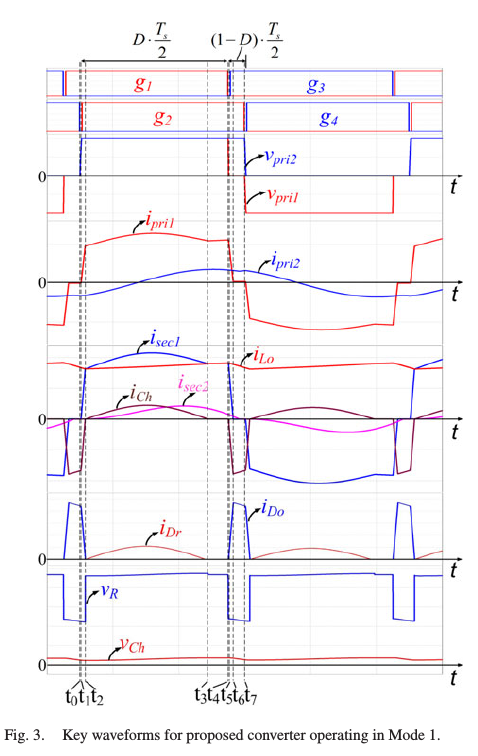
\includegraphics[scale=0.30]{key_waveforms.png}
	\end{figure}
	Yukaridaki grafikte 300, 360 ve 420V giris gerimleri icin verim ile cikis gucu arasindaki iliski verilmistir.
\end{frame}

\begin{frame}[fragile]{Kullanim Alanlari}
	\begin{itemize}
		\item Yuksek cikis voltajli uygulamalar
		\item Genis voltaj regulasyonu gerektiren uygulamar
		\item Onerilen yeni devre, elektrikli arac aku sarj uygulamasi icin yapilmistir.
	\end{itemize}
\end{frame}	

\plain{Sorular?}

\begin{frame}[allowframebreaks]{References}

  \bibliography{demo}
  \bibliographystyle{abbrv}

\end{frame}

\end{document}
